\subsection{Generating Candidate Patterns}
\label{GenPatterns}

Generating patterns to find new triplets serves as a crucial step in the extraction process of \emph{PPISnowball} system. Ideally, a perfect pattern should possess two properties: \emph{selectiveness},so that they barely coincide with incorrect tuples; and high \emph{coverage},so that they are representative enough to extract many new tuples\cite{Agichtein.Gravano:2000}.

\emph{PPISnowball} initially input a set of positive example tuples, for every protein$-$protein tuple $\langle protein\_1,protein\_2\rangle$, \emph{PPISnowball} find all context in whole document collections where protein\_1,protein\_2 and at least one interaction word occur in a sentence simultaneously by consulting the dictionaries mentioned in section \ref{DocumentPreprocessing}. \emph{PPISnowball} would replace proteins and interaction word with named-entity tags before analyze that sentence on the basis of certain rules (details later) to generate patterns. Taking the following sentence(PUBMED ID:12620407) as an example, \emph{PTEN regulates the transcriptional activity of p53 by modulating its DNA binding activity}. Since "PTEN" and "p53" are protein names, "regulates" indicates the interaction relationship between them, so the sentence after tagging looks like: \emph{$\langle PROT1\rangle$ $\langle INTERACTION\rangle$ the transcriptional activity of $\langle PROT2\rangle$ by modulating its DNA binding activity}.

Generally patterns are habitual language expressions that people tend to use to elaborate their ideas, either semantically or syntactically. A sufficiently-reliable pattern is expected to occur much more often in literatures than others do. According to such belief, we implement several patterns to measure habitual usage of language to describe a PPI information, next, we will briefly introduce their design principles.\\

\textbf{Shallow Linguistic Pattern. }  The \emph{Shallow Linguistic Pattern} is solely based on surface features (capitalization, punctuation, breaker,preposition, etc.) and shallow linguistic processing features (Part-of-Speech tagging and lemmatization). We borrow the feature set defined by Chowdhary for Bayesian Network building\cite{DBLP:journals/bioinformatics/ChowdharyZL09}. There are 12 features, which are strongly related to language rules. Using previous mentioned sentence as an example, \emph{PTEN regulates the transcriptional activity of p53 by modulating its DNA binding activity}. The pattern for triplet $\langle\langle PTEN,p53\rangle,regulates\rangle$ are the following: interactor,regulates; D1,0; D2,4; order,avb; prep,NA; conditional,n; comma, nn; but,n; which,n; not,n; breaker,n and NumberOfInteractors,high.

\textbf{Tri-Branch Part-Of-Speech(POS) Tree Pattern. } The \emph{Tri-Branch Part-Of-Speech(POS) Tree Pattern} is a subtree of the syntax tree (Figure \ref{fig:postree}A) generated by Stanford Parser (http://nlp.stanford.edu/software/lex-parser.shtml). When a syntax tree is acquired, since both proteins and interaction word are located in the leaf nodes of the tree, so we can backtrack the proteins and interaction word along the branches of the syntax tree until the root, thus obtain three routine respectively, after that,we can find a minimum(lowest-level) node which serve as the common ancestor of both proteins and interaction words (Figure \ref{fig:postree}B). Regarding the minimum common ancestor node as the new root, and three routine as new branches, here we get a subtree of original syntax tree (Figure \ref{fig:postree}C). What's more, for the sake of computational efficiency and representative neatness, we remove redundant elements, for example, the node directly above the protein is bound to a noun, in forms of "NN" or "NNP", so elimination of such information would do no harm to discrimination and uniqueness of patterns. Also we exert standardization on some tags, for example, there are many variation for a single verb tag, such as "VB" for base form, "VBZ" for 3rd person singular present, "VBD" for past tense, etc.To reduce ambiguity, we replace all related variation of verb with standard "VB" (Figure \ref{fig:postree}D).

\textbf{Tri-Branch Dependency Tree Pattern. } The \emph{Tri-Branch Dependency Tree Pattern} is a subtree of the collapsed dependency tree generated by Stanford Parser. In a dependency tree, nodes stand for words from sentence, and edges stand for grammatical relationship between words (Figure \ref{fig:deptree}A). However, the dependency tree cannot be used as pattern directly, for nodes are invariably different. Compared to nodes, the dependency relationship is much more stable and common, so we reverse the edges to nodes, in addition, we keep original protein and interaction word nodes (Figure \ref{fig:deptree}B). Finally, subtree rooted at minimum common ancestor is extracted based on the similar method mentioned by \emph{Tri-Branch Part-Of-Speech(POS) Tree Pattern}. Noticing that there won't necessarily be three routines in the subtree, for the reason that interaction word might hold a dominant position and thus become the ancestor of proteins (Figure \ref{fig:deptree}C).

%\begin{flushleft}
%\begin{figure}
%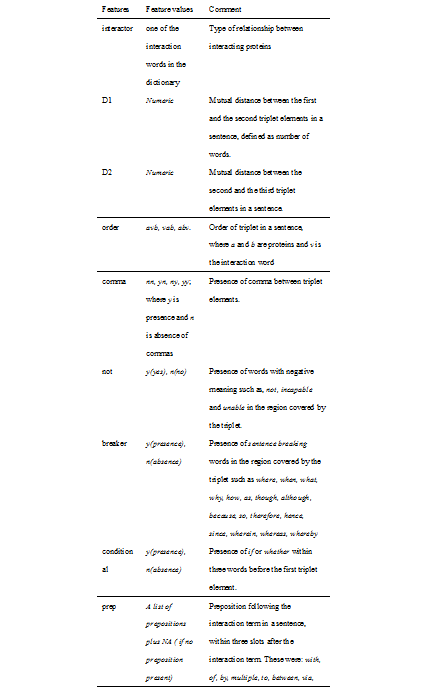
\includegraphics[width=100mm]{fig/figure3.png}
%\caption{Features used to encode protein-protein interaction rules in a sentence}
%\label{fig:feature}
%\end{figure}
%\end{flushleft}

\begin{flushleft}
\begin{figure}
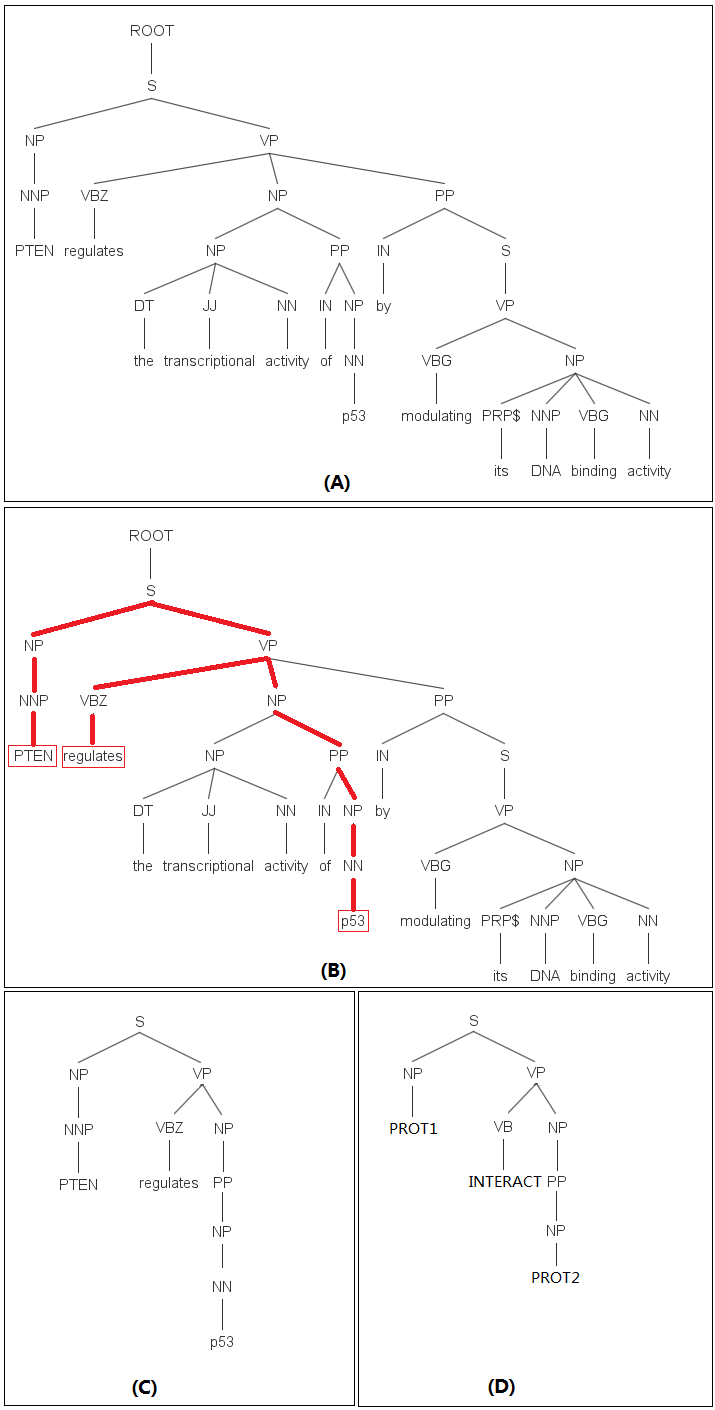
\includegraphics[width=80mm]{fig/figure5.png}
\caption{How a Tri-Branch Part-Of-Speech(POS) Tree Pattern generated. The example sentence is "\emph{PTEN regulates the transcriptional activity of p53 by modulating its DNA binding activity.}" \textbf{(A)} Original syntax tree generated by Stanford parser. \textbf{(B)} Find minimum common subtree where a pair of proteins and interaction word share the same ancestor. \textbf{(C)} Extract the minimum common subtree,with only three directly related branch kept. \textbf{(D)} Remove redundant POS tags as well as do tag standardization.}
\label{fig:postree}
\end{figure}
\end{flushleft}

\begin{flushleft}
\begin{figure}
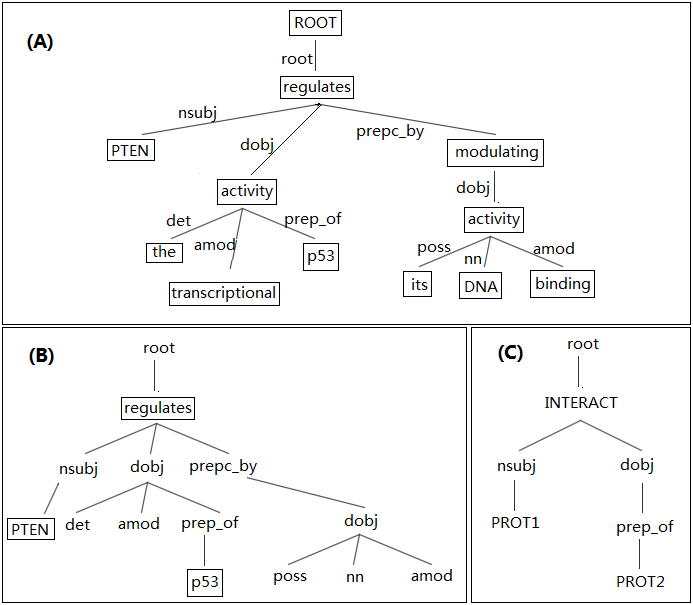
\includegraphics[width=80mm]{fig/figure6.png}
\caption{How a Tri-Branch Dependency Tree Pattern generated. The example sentence is "\emph{PTEN regulates the transcriptional activity of p53 by modulating its DNA binding activity.}" \textbf{(A)} Original dependency tree generated by Stanford parser. \textbf{(B)} Reverse the edge into nodes, in addition, keep original protein and interaction word nodes. \textbf{(C)} Prune none-directly related nodes and do tag standardization}
\label{fig:deptree}
\end{figure}
\end{flushleft}

\textbf{How to compare two distinct patterns. } In order to avoid replication of extracted patterns, a similarity function \emph{Sim(Pattern\_1,Pattern\_2)} is required to measure the distance between two patterns, of which the value belongs to [0,1]. The higher the value, the more similarity these two patterns hold. There are two kind of measure strategies, we will brief introduce their underlying principles as follows:

(1)\textbf{Rigid Similarity.} As the name implies, the rigid similarity focuses on total equality of two patterns. Either the two are exactly the same, then return 1 or they mismatch, then return 0. More specifically, for \emph{Shallow Linguistic Pattern}, only if all 12 features are identical would be regarded as the same; for \emph{Tri-Branch Part-Of-Speech(POS) Tree Pattern} or \emph{Tri-Branch Dependency Tree Pattern}, only if the extracted subtrees coincide would meet the requirement to be equal. Such all-or-nothing strategy is unsuitable to \emph{PPISnowball} system for it tends to result in low \emph{coverage}.

(2) \textbf{Soft Similarity.} Compared to rigid similarity, the soft similarity strategy is more flexible which would return a numeric number between 0 and 1. If the similarity score exceed some minimum similarity threshold $\mathcal {T}_{sim}$, then two patterns would be regarded as the same. Though seemingly promising, it still remains challenge to implement a proper soft similarity strategy. We would introduce graph kernel in detail later (Section \ref{AugmentPatterns}).


